\documentclass[a4paper,12pt]{report}
\usepackage{algorithmic}
\usepackage[linesnumbered,ruled,vlined]{algorithm2e}
\usepackage[margin=2cm]{geometry}
\usepackage[utf8]{inputenc}
\usepackage{listings} 
\usepackage{graphicx} 
\usepackage{color}
\usepackage{xcolor}
\usepackage{hyperref}
%\usepackage{mdframed}

\newcommand\tab[1][1cm]{\hspace*{#1}}
\graphicspath{ {images/} }
\newcommand{\currentdata}{ 1 February 2017}
\newtheorem{example}{Example}

\begin{document}
\vspace{-5cm}
\begin{center}
Department of Computer Science\\
Technical University of Cluj-Napoca\\

\includegraphics[width=10cm]{fig/footer}
\end{center}
\vspace{1cm}
%\maketitle
\begin{center}
\begin{Large}
 %\textbf{Introduction to Artificial Intelligence}\\
\textbf{Intelligent Systems}\\
\end{Large}
\textit{Laboratory activity 2016-2017}\\
\vspace{3cm}
Adrian Groza, Anca Marginean and Radu Razvan Slavescu\\
Tool: Machine learning- neural networks sckit-learn\\
\vspace{1.5cm}
Name:Brincoveanu Vasile Vlad si Ghiurca Dorin\\
Group:30233\\
Email:gg.vladbrincoveanu@gmail.com\\
\vspace{6cm}
Assoc. Prof. dr. eng. Adrian Groza\\
Adrian.Groza@cs.utcluj.ro\\
\vspace{1cm}

\includegraphics[width=10cm]{fig/footer}
\end{center}

\tableofcontents


%\chapter{Laboratory works}

\chapter{Installing the tool ($W_1$)}

\colorbox{blue!20}{\fbox{\begin{minipage}{1.0\textwidth}                                  
The teaching objectives for this week are:
\begin{enumerate}
 \item To know how to use the tool in our future project.
\item To know from where we can download it, what version, etc. And how to run it.
\end{enumerate}
\end{minipage}}}\\

\colorbox{blue!20}{\fbox{\begin{minipage}{16cm}Steps for installing the tool on windows or mac:
\begin{enumerate}
\item First step is to go on the \href{http://www.scikit-learn.org/}{application site}
\item Then you need to go on the installation part of the site.
\item Under installing the latest release section it can be found the linux commands for installing scikit-learn prerequisites.
\end{enumerate}
\end{minipage}}}\\

\begin{itemize}
\item
	\tab Some notes: you should have python (2.7-eq. or greater, or 3.3 - eq. or greater), NumPy (1.8.2 - eq. or greater), SciPy(0.13.3 - eq.  or greater) installed prior to  running the application, otherwise it won't work.\\

\end{itemize}

\chapter{Running and understanding examples ($W_2$)}
\colorbox{blue!20}{\fbox{\begin{minipage}{1.0\textwidth}                                  
The teaching objectives for this week are:
\begin{enumerate}
 \item To run and understand the some examples.
\item To identify what realistic problems are adequate for our tool. 
\end{enumerate}
\end{minipage}}}
\graphicspath{ {fig/} }
\begin{itemize}
\item{First example}

\tab We can use scikit-learn to recognize images of hand-written digits.

\begin{center}
  	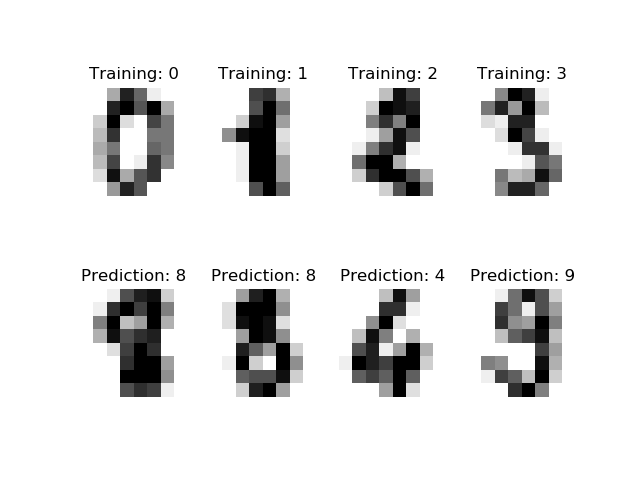
\includegraphics[scale=0.8]{exemplu1}
\end{center}

\begin{lstlisting}[frame=single]
"""
================================
Recognizing hand-written digits
================================

An example showing how the scikit-learn can be used to recognize 
images of hand-written digits.

This example is commented in the
:ref:`tutorial section of the user manual <introduction>`.

"""
print(__doc__)

# Author: Gael Varoquaux <gael dot varoquaux at normalesup dot 
org>
# License: BSD 3 clause

# Standard scientific Python imports
import matplotlib.pyplot as plt

# Import datasets, classifiers and performance metrics
from sklearn import datasets, svm, metrics

# The digits dataset
digits = datasets.load_digits()

# The data that we are interested in is made of 8x8 images of 
#digits, let's  have a look at the first 4 images, stored in the 
#`images` attribute of the dataset.  If we were working from
# image files, we could load them using matplotlib.pyplot.imread.  
#Note that each image must have the same size. For these
# images, we know which digit they represent: it is given in the 
#'target' of the dataset.
images_and_labels = list(zip(digits.images, digits.target))
for index, (image, label) in enumerate(images_and_labels[:4]):
    plt.subplot(2, 4, index + 1)
    plt.axis('off')
    plt.imshow(image,cmap=plt.cm.gray_r,interpolation='nearest')
    plt.title('Training: %i' % label)

# To apply a classifier on this data, we need to flatten the 
#image, to turn the data in a (samples, feature) matrix:
n_samples = len(digits.images)
data = digits.images.reshape((n_samples, -1))

# Create a classifier: a support vector classifier
classifier = svm.SVC(gamma=0.001)

# We learn the digits on the first half of the digits
classifier.fit(data[:n_samples //2],digits.target[:n_samples //2])

# Now predict the value of the digit on the second half:
expected = digits.target[n_samples // 2:]
predicted = classifier.predict(data[n_samples // 2:])

print("Classification report for classifier %s:\n%s\n"
      % (classifier, metrics.classification_report(expected, predicted)))
print("Confusion matrix:\n%s" % metrics.confusion_matrix(expected, predicted))

images_and_predictions = list(zip(digits.images[n_samples // 2:], predicted))
for index, (image, prediction) in enumerate(images_and_predictions[:4]):
    plt.subplot(2, 4, index + 5)
    plt.axis('off')
    plt.imshow(image, cmap=plt.cm.gray_r, interpolation='nearest')
    plt.title('Prediction: %i' % prediction)

plt.show()

\end{lstlisting}

\item{Second example - Linear Regression}

\tab This example uses the only the first feature of the diabetes dataset, in order to illustrate a two-dimensional plot of this regression technique. The straight line can be seen in the plot, showing how linear regression attempts to draw a straight line that will best minimize the residual sum of squares between the observed responses in the dataset, and the responses predicted by the linear approximation.

The coefficients, the residual sum of squares and the variance score are also calculated.\\

\begin{center}
  	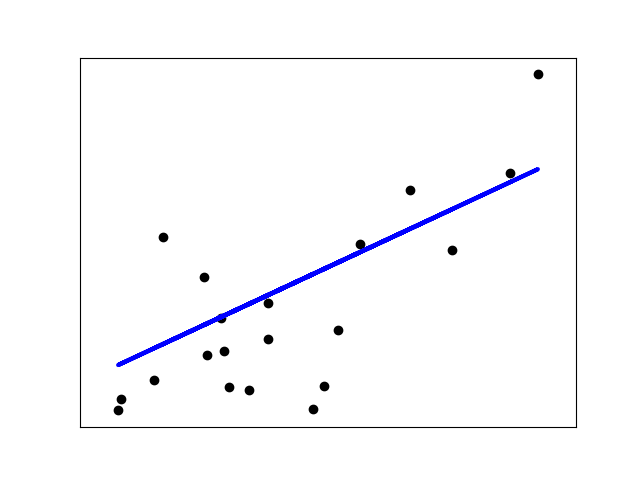
\includegraphics[scale=0.8]{exemplu2}
\end{center}

\begin{lstlisting}[frame=single]
print(__doc__)


# Code source: Jaques Grobler
# License: BSD 3 clause


import matplotlib.pyplot as plt
import numpy as np
from sklearn import datasets, linear_model
from sklearn.metrics import mean_squared_error, r2_score

# Load the diabetes dataset
diabetes = datasets.load_diabetes()


# Use only one feature
diabetes_X = diabetes.data[:, np.newaxis, 2]

# Split the data into training/testing sets
diabetes_X_train = diabetes_X[:-20]
diabetes_X_test = diabetes_X[-20:]

# Split the targets into training/testing sets
diabetes_y_train = diabetes.target[:-20]
diabetes_y_test = diabetes.target[-20:]

# Create linear regression object
regr = linear_model.LinearRegression()

# Train the model using the training sets
regr.fit(diabetes_X_train, diabetes_y_train)

# Make predictions using the testing set
diabetes_y_pred = regr.predict(diabetes_X_test)

# The coefficients
print('Coefficients: \n', regr.coef_)
# The mean squared error
print("Mean squared error: %.2f"
      % mean_squared_error(diabetes_y_test, diabetes_y_pred))
# Explained variance score: 1 is perfect prediction
print('Variance score: %.2f' % r2_score(diabetes_y_test, diabetes_y_pred))

# Plot outputs
plt.scatter(diabetes_X_test, diabetes_y_test,  color='black')
plt.plot(diabetes_X_test, diabetes_y_pred, color='blue', linewidth=3)

plt.xticks(())
plt.yticks(())

plt.show()
\end{lstlisting}

\end{itemize}
 
\chapter{Understanding conceptual instrumentation ($W_3$)}
\label{ch:tool}

\colorbox{blue!20}{\fbox{\begin{minipage}{1.0\textwidth}                                  
The teaching objectives for this week are:
\begin{enumerate}
 \item  To understand the algorithm(s) on which your tool relies.
\item To get used with writing algorithms in Latex
\end{enumerate}
\end{minipage}}}\\

\begin{itemize}
\item{Explaining the tool}

\tab Machine learning algorithms implemented in scikit-learn expect data to be stored in a two-dimensional array or matrix. The arrays can be either numpy arrays, or in some cases scipy.sparse matrices. The size of the array is expected to be: [n samples, n features]. \\ 

\tab scikit-learn comes with a few standard datasets, for instance the iris and digits datasets for classification and the boston house prices dataset for regression. A dataset is a dictionary-like object that holds all the data and some metadata about the data. This data is stored in the .data member, which is a n samples, n features array. In the case of supervised problem, one or more response variables are stored in the .target member. More details on the different datasets can be found in the dedicated section.\\

\tab In the case of the digits dataset, the task is to predict, given an image, which digit it represents. We are given samples of each of the 10 possible classes (the digits zero through nine) on which we fit an estimator to be able to predict the classes to which unseen samples belong.

In scikit-learn, an estimator for classification is a Python object that implements the methods fit(X, y) and predict(T).\\

\end{itemize}

\chapter{Project description ($W_4$)}


\colorbox{blue!20}{\fbox{\begin{minipage}{1.0\textwidth}                                  
The teaching objectives for this week are:
\begin{enumerate}
 \item To have a clear description of what you intend to develop.
\item To point to specific resources (datasets, knowledge bases, external tools) 
that support the development of your idea and which minimise the risk of failure.
\item To identify related work (articles) that are relevant or similar to your approach.
\end{enumerate}
\end{minipage}}}\\

\section{Describe in natural language}

\tab We propose to predict the chance of having a heart disease or having hypertension given the dataset.\\
\tab Our approach was to use neural networks and to try different algorithms integrated in Multi-layer Perceptron (MLP) and compare which one of those works better for the given dataset of heart disease. More detailed info will be described in implementation chapter.\\

\tab We will start by examinin our dataset .\footnote{https://www.kaggle.com/asaumya/healthcare-problem-prediction-stroke-patients} . The datasets are provided by SaumyaAgarwal HealthCare Problem: Prediction Stroke Patients on the kaggle website. He used it to predict stroke by having different data. We will use it for predicting  heart disease or having hypertension.\\

\tab Understanding Data
Here is the Definitions of the columns of the data

id-Patient ID\\
gender-Gender of Patient\\
age-Age of Patient\\
hypertension-0 - no hypertension, 1 - suffering from hypertension\\
heart-disease-0 - no heart disease, 1 - suffering from heart disease\\
ever-married-Yes/No\\
work-type-Type of occupation\\
Residence-type-Area type of residence (Urban/ Rural)\\
avg-glucose-level-Average Glucose level (measured after meal)\\
bmi-Body mass index\\
smoking-status-patient’s smoking status\\
stroke-0 - no stroke, 1 - suffered stroke\\

\tab The columns that we will be using are all except id-patient and stroke, to not interfere with what our poster used the data for.\\
\tab Furthermore, there are 2 datasets, one for training and one for testing. We merged all , and use cross-validation function to split the data into test data and train data.\\

\tab All this data will be converted to integers, usign different functions of the panda library.\\ 

\chapter{Algorithms ($W_8$)}

\begin{itemize}
\item{Neural network models}

\tab Multi-layer Perceptron (MLP) is a supervised learning algorithm that learns a function f(dot): R to the power m goest to  R to the power o by training on a dataset, where m is the number of dimensions for input and o is the number of dimensions for output. Given a set of features X = {x1, x2, ..., xm} and a target y, it can learn a non-linear function approximator for either classification or regression. It is different from logistic regression, in that between the input and the output layer, there can be one or more non-linear layers, called hidden layers. Figure 1 shows a one hidden layer MLP with scalar output. \\ 

\tab The advantages of Multi-layer Perceptron are:

	- capability to learn non-linear models.

	- capability to learn models in real-time (on-line learning) using partial fit.

The disadvantages of Multi-layer Perceptron (MLP) include:

	- MLP with hidden layers have a non-convex loss function where there exists more than one local minimum. Therefore different random weight initializations can lead to different validation accuracy.

	- MLP requires tuning a number of hyperparameters such as the number of hidden neurons, layers, and iterations.

	- MLP is sensitive to feature scaling.  \\

\item{Classifier}

\tab Class MLPClassifier implements a multi-layer perceptron (MLP) algorithm that trains using Backpropagation.

MLP trains on two arrays: array X of size (n samples, n features), which holds the training samples represented as floating point feature vectors; and array y of size (n samples,), which holds the target values (class labels) for the training samples. \\

\tab  Currently, MLPClassifier supports only the Cross-Entropy loss function, which allows probability estimates by running the predict proba method.

MLP trains using Backpropagation. More precisely, it trains using some form of gradient descent and the gradients are calculated using Backpropagation. For classification, it minimizes the Cross-Entropy loss function, giving a vector of probability estimates P(y|x) per sample x. \\

\tab  MLPClassifier supports multi-class classification by applying Softmax as the output function.

Further, the model supports multi-label classification in which a sample can belong to more than one class. For each class, the raw output passes through the logistic function. Values larger or equal to 0.5 are rounded to 1, otherwise to 0. For a predicted output of a sample, the indices where the value is 1 represents the assigned classes of that sample. \\

\end{itemize}

\chapter{Implementation details ($W_5$)}

The teaching objectives for this week are:
\begin{enumerate}
 \item Illustrate each aspect of the reality that you have 
 modelled in your solution.
\item To explain the relevant code from your scenario.
\end{enumerate}

\section{Start example}
\tab We will model the network by startting from an example which can be found \href{https://www.norsys.com/tutorials/netica/secA/tut_A1.html}{here} where is described a case for some diseases.\\

\section{How we chose nodes}
\tab Nodes will be chosen by the chosen scope. We will put a diagnosis of a person who walks to a clinic and presents fever, vomiting, muscle pain, eec. We will try to determine the disease of the pacient by these. Nodes 
will be chosen such that it will have a bigger spectre of posibilities.\\

\section{Probabilities}

\tab To calculate the probability of having fever, the logical "noisy" relationships are used. In propositional logic we can say that fever is true if and only if malaria, yellow fever or flu are true. The noisy-OR model allows for uncertainties as to the ability of each parent to cause his descendant to be true, so a person may have flu but without fever.\\
\tab The model assumes that anything that inhibits a parent to produce a child's effect is independent of any inhibition by other parents to produce offspring effects: for example, any inhibit malaria to cause fever is independent of any flu inhibiting to produce fever. With these assumptions, fever has the false value if and only if all of his parents are inhibited to produce fever, and the probability is the product of inhibition probabilities q for each parent. We assume the following probability of inhibition:\\
\begingroup\makeatletter\def\@currenvir{verbatim}
\verbatim
q_gripa = p(-febra|gripa, -malarie, -febra g) = 0.6;
q_febra g = p(-febra |-gripa, malarie, febra g) = 0.1;
q_malarie  = p(-febra |gripa, malarie, -febra g) = 0.1;
Pe baza acestor informatii si ale asumptiilor noisy-OR,
 se poate construi tabelul de probabilitati de mai sus. Regula generala este:
	P(x_i | parents(X_i)) = 1 – product (given that j:X_j = true)[q_j], 
unde produsul este aplicat parintilor care au valoarea true pentru randul respectiv.

p(febra|malarie) = 1 – q_malarie = 1 – 0.15 = 0.85  
p(febra|febra galbena) = 1 – q_febraGalbena = 1 – 0.1 = 0.9
p(febra|malarie, febra galbena) = 1   - q_malarie,febraGalbena =
 true = 1 – (0.15 * 0.1) = 0.985
p(febra|gripa) = 1 – q_gripa = 1-0.6 = 0.4
p(febra|gripa, febra galbena) = 1 – q_gripa,febraGalbena =
 true = 1 – (0.6 * 0.1) = 0.94
p(febra|gripa, malarie) = 1 – q_gripa,malarie = true   =
 1 – (0.6 * 0.15) = 0.91
p(febra|gripa,malarie,febra galbena) = 1 – q_gripa,malarie,
febra galbena = true = 1 – (0.6*0.1*0.15) = 0.991.

In cazul laringitei, valorile sunt urmatoarele:
q_contact_persoane_bolnave = p(-laringita |
 contact persoane bolnave, -consum tutun/alcool) = 0.22.
q_consum_tutun/alcool = p(-laringita | -contact cu persoane bolnave,
 consum tutun/alcool) = 0.6.

p(laringita | -contact cu persoane bolnave, -consum_tutun/alcool) = 0
p(laringita | consum tutun/alcool) = 1 – q_consum_tutun/alcool=true    = 
 1 – 0.6 = 0.4
p(laringita | contact cu persoane bolnave = 1 – q_contact_persoane_bolnave =
 true   =   1 – 0.22 = 0.78
p(laringita | contact cu persoane bolnave, contact cu persoane bolnave) =
 1 – (0.66 * 0.22) = 0.868.

In cazul starilor de voma, valorile sunt urmatoarele:

q_malarie = p(-stari de voma | malarie, -febra galbena) = 0.34
q_febraGalbena = p(-stari de voma | -malarie, febra galbena) = 0.43

p(stari de voma | -malarie, -febra galbena) = 0
p(stari de voma | -malarie, febra galbena) = 1 – q_febraGalbena = true   =

  1 – 0.43 = 0.57
p(stari de voma | malarie, -febra galbena) = 1 – q_malarie=true   = 1 – 0.34 = 0.66
p(stari de voma | malarie, febra galbena)  = 1 – q_malarie, febraGalbena=true  = 
1  - (0.34 * 0.43) = 0.8538


 In cazul pneumoniei, valorile sunt urmatoarele:
q_gripa = p(-pneumonie | gripa) = 0.28
p(pneumonie | -gripa) = 0.1
p(pneumonie | gripa) = 1  - q_gripa=true   = 1 – 0.28  = 0.72


In cazul tuselor/problemelor respiratorii, valorile sunt urmatoarele:
q_gripa = p(-probleme respiratorii | gripa, -laringita)  = 0.57
q_laringita = p(-probleme respiratorii | -gripa, laringita) = 0.04

p(probleme respiratorii| - laringita, -gripa) = 0
p(probleme respiratorii | -gripa, laringita) = 1 – q_laringita=true  =
 1 – 0.04 = 0.96
p(probleme respiratorii | gripa, -laringita) = 1  - q_gripa=true =
 1 -  0.57 = 0.43
p(probleme respiratorii | gripa, laringita) =1 – q_gripa,laringita=true  = 
1 – (0.57 * 0.04) = 0.9772

In cazul comei, valorile sunt urmatoarele:
q_malarie = p(-coma|malarie) = 0.91
p(coma|malarie) = 1 – q_malarie=true   = 1 – 0.91 = 0.09
p(coma|-malarie) = 0


In case of death, probabilities are the following:
q_febraGalbena = q(-moarte | febraGalbena, -malarie, -laringita, -gripa)  = 0.999992
q_malarie = q(-moarte | -febraGalbena, malarie, -laringita, -gripa)  = 0.9712
q_laringita = q(-moarte | -febraGalbena, -malarie, laringita, -gripa)  = 0.9999993
q_gripa = q(-moarte | -febraGalbena, -malarie, -laringita, gripa)  = 0.999992

p(moarte | -febraGalbena, -malarie, -laringita, -gripa)  = 0
p(moarte | febraGalbena, malarie, laringita, gripa)  = 1 -q_all=true = 
1 – (0.999992 * 0.9712 * 0.9999993 * 0.999992) = 0.0288
p(moarte | febraGalbena, malarie, laringita)  = 1 -q_fg,malarie, laringita=true   = 
 1 – (0.999992 * 0.9712 * 0.9999993) = 0.0288
p(moarte | febraGalbena, malarie, gripa)  = 1 -q_fg,m,g=true  =
 1 – (0.999992 * 0.9712 * 0.999992) = 0.028815
p(moarte | febraGalbena, malarie)  = 1 -q_fg,m = 1 – (0.999992 * 0.9712) = 0.028807
p(moarte | febraGalbena, laringita, gripa)  = 1 – q_fg,l,g=true   = 
  1 – (0.999992 * 0.9999993 * 0.999992) = 0.000008
p(moarte | febraGalbena, laringita)  = 1 – q_fg,l=true   =  
 1 – (0.999992 * 0.9999993) = 0.000008
p(moarte | febraGalbena)  = 1 – q_fg=true   =   1 – 0.999992 = 0.000008
p(moarte | malarie, laringita, gripa)  = 1 -q_m,l,g=true =
 1 – (0.9712 * 0.9999993 * 0.999992) = 0.02880
p(moarte | malarie, laringita)  = 1 -q_m,l,g=true = 1 – (0.9712 * 0.9999993) = 0.0288
p(moarte | malarie, gripa)  = 1 -q_m,g=true = 1 – (0.9712 * 0.9999992) = 0.0288
p(moarte | malarie)  = 1 -q_m=true = 1 – (0.9712) = 0.0288
p(moarte | laringita, gripa)  = 1 -q_l,g=true = 
1 – (0.9999993 * 0.9999992) = 0.000008
p(moarte | laringita)  = 1 -q_l,g=true = 1 – (0.9999993) = 0.000008


\end{verbatim}

\chapter{Experiments and tables ($W_{6}$)}

The objectives for this week are:
\begin{enumerate}
 \item To describe and interpret each experiment that you have performed
\end{enumerate}

An experiment investigates how some variables are related. 
Usually, experiments verify a previosly formulated hypothesis.
Such hypothesis may investigate how your software degrades its performance with larger inputs.
You will need to run simulations to see how your implementation is affected by different inputs.

\section{Result interpretation and data}

\tab Here we will put all the results regarding hypertension and heart-disease from our dataset. We tested it with neural networks, with different algs and with lienarSCV and SCV ot see the diferences. \\
\tab The dataset percentage refeers to the amount of true test data in the dataset. If we let all the rows of the dataset, we will see that every classifier will predict false negative, and false positive, because there is few people with hypertension.\\
\tab We will manipulate the dataset in our favor, to be more precise in thesting the algorithms.\\


\tab Precision (also called positive predictive value) is the fraction of relevant instances among the retrieved instances, while recall (also known as sensitivity) is the fraction of relevant instances that have been retrieved over the total amount of relevant instances.Wiki.\\

\tab The F1 score is the harmonic average of the precision and recall, where an F1 score reaches its best value at 1 (perfect precision and recall) and worst at 0.\\

\tab ‘lbfgs’ is an optimizer in the family of quasi-Newton methods.\\
\tab ‘sgd’ refers to stochastic gradient descent.\\
\tab adam’ refers to a stochastic gradient-based optimizer proposed by Kingma, Diederik, and Jimmy Ba\\


\tab \tab \textbf{Confusion matrix}
\begin{center}
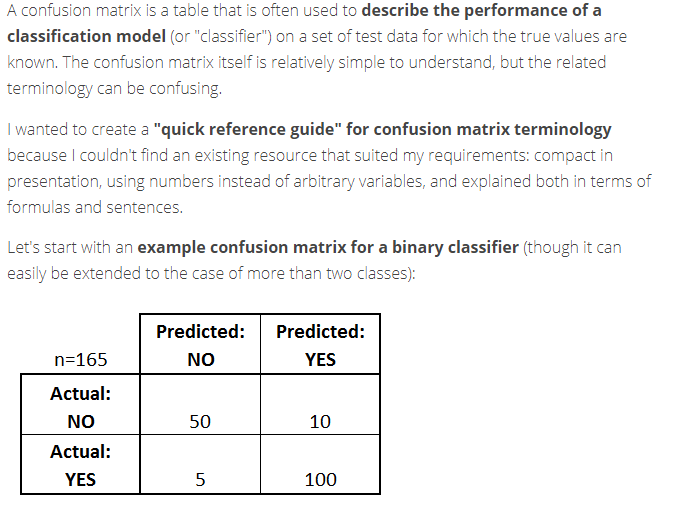
\includegraphics[scale=0.65]{confmatrix.png}
\end{center}

\begin{table}[h!]
\begin{center}
\caption{Results for predicting hypertension}
\label{tab:table1}
\begin{tabular}{c c c c c}
\textbf{Method and algorithm} & \textbf{Dataset percentage(true)} & \textbf{Precision }& \textbf{Recall }& \textbf{F1-score }\\
\hline
Neural Net - lbfgs & 45.6 & 0.69 & 0.69 & 0.69\\
Neural Net - lbfgs & 54.11 & 0.58 & 0.54 & 0.39\\
Neural Net - sgd & 45.6 & 0.53 & 0.52 & 0.38\\
Neural Net - sgd & 54.11 & 0.50 & 0.54 & 0.39\\
Neural Net - adam & 45.6 & 0.57 & 0.53 & 0.37 \\
Neural Net - adam & 54.11 & 0.58 & 0.50 & 0.42 \\
All data NN-adam & 0.09 & 0.82 & 0.89 & 0.83 \\
\end{tabular}
\end{center}
\end{table}

\begingroup\makeatletter\def\@currenvir{verbatim}
\verbatim
 Where confusion matrix of 1.\\
\[414, 157\],\\
\[183, 338\]\\

\tab confusion matrix of 2.\\
\[ 7, 395\],\\
\[ 4, 461\]\\

\tab confusion of 3.
\[558, 13\],\\
\[506, 15\]\\

\tab confusion of 4.
\[ 6, 396\],\\
\[ 7, 458\]\\

\tab conf of 5.
\[566, 5\],\\
\[513, 8\]\\

\tab conf of 6.
\[368, 34\]\\
\[397, 68\]\\
\end{verbatim}


\tab Here we see that there is a kind of good prediction , regarding the small sample of the dataset. Ofc, if we were to put all 50k rows in we will get 95 per cent prediction but only because the neural network have been trained to predict all values false because of dataset having few 5-10 per cent values of true in the test data.\\


\begin{table}[h!]
\begin{center}
\caption{Results for predicting heart-disease}
\label{tab:table2}
\begin{tabular}{c c c c c} 
\textbf{Method and algorithm} & \textbf{Dataset percentage(true)} & \textbf{Precision }& \textbf{Recall }& \textbf{F1-score }\\
\hline
Neural Net - lbfgs & 45.6 & 0.41 & 0.64 & 0.50 \\
Neural Net - lbfgs & 54.11 & 0.53 & 0.73 & 0.61 \\
Neural Net - sgd & 45.6 & 0.63 & 0.64 & 0.51\\
Neural Net - sgd & 54.11 & 0.62 & 0.73 & 0.61\\
Neural Net - adam & 45.6 & 0.66 & 0.44 & 0.37 \\
Neural Net - adam & 54.11 & 0.67 & 0.73 & 0.64 \\
All data NN-adam & 0.09 & 0.91 & 0.95 & 0.93 \\
\end{tabular}
\end{center}
\end{table}


\begingroup\makeatletter\def\@currenvir{verbatim}
\verbatim
Where confusion matrix of 1.\\
\[411, 0\],\\
\[233, 0\]\\

\tab confusion matrix of 2.\\
\[632, 0\],\\
\[237, 0\]\\

\tab confusion of 3.
\[409, 2\],\\
\[230, 3\]\\

\tab confusion of 4.
\[630, 2\],\\
\[236, 1\]\\

\tab conf of 5.
\[ 67, 344\],\\
\[ 16, 217\]\\

\tab conf of 6.
\[617, 15\],\\
\[223, 14\]\\

\tab conf of 7.
\[3554, 1\],\\
\[ 172, 0\]\\

\end{verbatim}



\section{Conclusions}

\tab The default solver ‘adam’ works pretty well on relatively large datasets (with thousands of training samples or more) in terms of both training time and validation score. For small datasets, however, ‘lbfgs’ can converge faster and perform better.Skit.\\

\tab Here we see that there is a kind of good prediction , regarding the small sample of the dataset. Ofc, if we were to put all 50k rows in we will get 95 per cent prediction but only because the neural network have been trained to predict all values false positive because of dataset having few 5-10 per cent values of true in the test data.\\

\tab One fact, if we add hidden layers of neurons, the values will start to converge rapidily to 80+ prediction and go into false positive values, like we said in the upper paragraph.\\

\chapter{Related Work}

\begin{itemize}
\item{Approach}

\tab Our approach was to try different classifier and try and compare which one of those works better for the given dataset of heart disease. The classifiers that we have compared are Linear SVM, Non-linear SVM and Stratified K-Mean on the given vector representation of Cleveland dataset. For our experimental purposes, we have divided our experiment into 2 problems. For both problems, we try to run our classifiers for 60/40 and 80/20 splits where we use 60 per cent and 80 per cent for training our classifiers and 40 per cent  and 20 percent for testing their predictions respectively. Cleveland dataset  has 303 instances and 14 attributes. Our first step is to apply dimensionality reduction and for that purpose we have use Principal Component Analysis (PCA) with 5 components. Once the PCA has been applied on the original X value where X is the feature set, our feature set is reduced to X-new which is a vector representation of 303 samples x 5 features.  First, we try out 60/40 split of X-new where 60 per cent of X-new is used to train the SVM classifier and 40 per cent of X-new is used to test. Similarly, next we try 80/20 split of X-new, which is problem 1 of our experiment. \\

\item{Problem 1}

\tab We classify data using a Linear SVM and predict likelihood of disease belonging to a particular class of severity ranging from 1 to 4 i.e. least to most severe with value of C=0.001. Here, C is the penalty that the classifier incurs every time there is a misclassification that takes place so job of the classifier is to incur penalty as minimal as possible while classifying data in order to keep cost of classification at minimum. In order to check if other type of classifiers work better for this dataset than Linear SVM, we use a RBF i.e. non-linear kernel for the SVM classifier and classify data keeping value of C same. Similarly as last part of our problem 1, we use Stratified k-fold cross validation with 5 folds with a RBF kernel and keeping value of C same as for above classifiers in our search to find which classifier works better for this dataset. The results for this have been shown below in Fig 1 below. \\

\item{Problem 2}

\tab For problem-2 of our experiment, we go a step further by predicting absence (zero) or presence (non-zero) of heart disease. This is possible because we group all severity classes (1 to 4) together which mean that a non-zero would indicate presence of heart disease and a zero would indicate absence of heart disease. Problem-2 of the experiment follows same procedure as that of problem-1. First step is dimensionality reduction for which we use PCA with 5 components that picks best 5 components out of 14 attributes. Now what we get is a vector representation as we obtained in problem-1, which basically implies 303 samples x 5 features. For problem-2, we use an 80/20 split where 80 per cent of data is used to train classifier and 20 per cent is used to test. Now, we follow the same procedure as we did for problem-1 we apply 3 classifiers i.e. Linear SVM, Non-Linear SVM with RBF kernel and Stratified k-means cross validation with 5 folds, all for a value of C=0.001. The results are shown in fig.2. \\

\item{Results}

\begin{center}
  	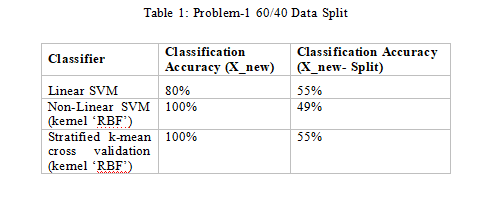
\includegraphics[scale=0.8]{tabel1.png}
\end{center}

\begin{center}
  	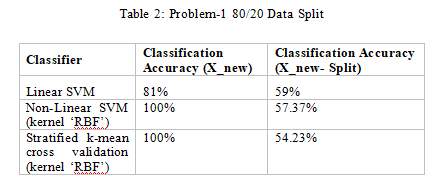
\includegraphics[scale=0.8]{tabel2.png}
\end{center}

\begin{center}
  	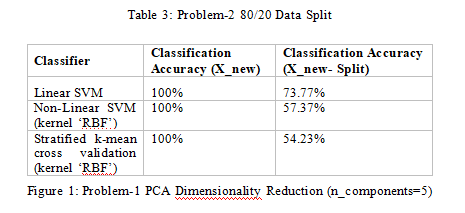
\includegraphics[scale=0.8]{tabel3.png}
\end{center}

\begin{center}
  	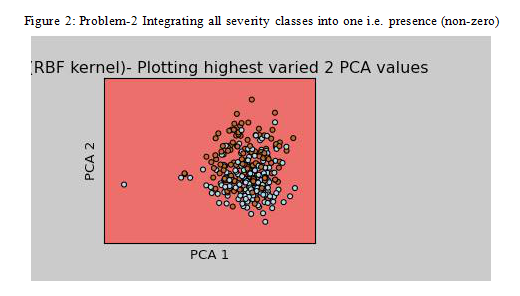
\includegraphics[scale=0.8]{rezultat1.png}
\end{center}

\item{Conclusion}

\tab Based on the results shown above and experiments performed, it is evident that input data plays an important role in prediction along with machine learning techniques. As is seen in the dataset, provided, we have labels from 0 to 4 where the labels of 4 are hardly 13 and when we split the data into train and test, the number become very less which is nothing but noise and can be totally removed from the dataset by using filtering techniques and hence the linear model will be available to predict the outcome much better with absence of noise. Moreover, PCA has again proven that we can get rid of similar feature set and still obtain predictions with great efficiency. Moreover, we have conducted tests using non linear RBF kernel which is a normal first choice and then validating against linear SVC kernel which outperformed RBF in split case. Most importantly, the above experiment not only helped us in predicting the outcome but also gave us valuable insights about the nature of data, which can be used in future to train our classifiers in a much better way. \\

\tab All source file can be founded  \href{https://github.com/diwakar02/Heart-Disease-Prediction-using-Machine-Leaning}{here.}\\

\end{itemize}

\appendix

\chapter{Your original code}
\label{app:code}

\begingroup\makeatletter\def\@currenvir{verbatim}
\verbatim

<?xml version="1.0" encoding="UTF-8"?>
<BIF VERSION="0.3"  xmlns="http://www.cs.ubc.ca/labs/lci/fopi/ve/XMLBIFv0_3"
	xmlns:xsi="http://www.w3.org/2001/XMLSchema-instance"
	xsi:schemaLocation="http://www.cs.ubc.ca/labs/lci/fopi/ve/XMLBIFv0_3
 http://www.cs.ubc.ca/labs/lci/fopi/ve/XMLBIFv0_3/XMLBIFv0_3.xsd">
<NETWORK>
<NAME>Untitled</NAME>
<PROPERTY>detailed = </PROPERTY>
<PROPERTY>short = </PROPERTY>

<VARIABLE TYPE="nature">
	<NAME>Vizita Africa</NAME>
	<OUTCOME>T</OUTCOME>
	<OUTCOME>F</OUTCOME>
	<OBS>T</OBS>
	<PROPERTY>position = (7291.9384765625, 5058.5302734375)</PROPERTY>
</VARIABLE>

<VARIABLE TYPE="nature">
	<NAME>Stari de voma</NAME>
	<OUTCOME>T</OUTCOME>
	<OUTCOME>F</OUTCOME>
	<PROPERTY>position = (7193.0849609375, 5296.3046875)</PROPERTY>
</VARIABLE>

<VARIABLE TYPE="nature">
	<NAME>Contact cu persoane bolnave</NAME>
	<OUTCOME>T</OUTCOME>
	<OUTCOME>F</OUTCOME>
	<PROPERTY>position = (7511.494140625, 5050.837890625)</PROPERTY>
</VARIABLE>

<VARIABLE TYPE="nature">
	<NAME>Consum alcool/tutun</NAME>
	<OUTCOME>T</OUTCOME>
	<OUTCOME>F</OUTCOME>
	<PROPERTY>position = (7766.93310546875, 5048.2373046875)</PROPERTY>
</VARIABLE>

<VARIABLE TYPE="nature">
	<NAME>Malarie</NAME>
	<OUTCOME>T</OUTCOME>
	<OUTCOME>F</OUTCOME>
	<OBS>T</OBS>
	<PROPERTY>position = (7193.0791015625, 5194.01123046875)</PROPERTY>
</VARIABLE>

<VARIABLE TYPE="nature">
	<NAME>Febra galbena</NAME>
	<OUTCOME>T</OUTCOME>
	<OUTCOME>F</OUTCOME>
	<OBS>T</OBS>
	<PROPERTY>position = (7382.18896484375, 5191.4443359375)</PROPERTY>
</VARIABLE>

<VARIABLE TYPE="nature">
	<NAME>Gripa</NAME>
	<OUTCOME>T</OUTCOME>
	<OUTCOME>F</OUTCOME>
	<PROPERTY>position = (7549.552734375, 5189.99951171875)</PROPERTY>
</VARIABLE>

<VARIABLE TYPE="nature">
	<NAME>Laringita</NAME>
	<OUTCOME>T</OUTCOME>
	<OUTCOME>F</OUTCOME>
	<OBS>F</OBS>
	<PROPERTY>position = (7716.47705078125, 
5183.78759765625)</PROPERTY>
</VARIABLE>

<VARIABLE TYPE="nature">
	<NAME>Febra</NAME>
	<OUTCOME>T</OUTCOME>
	<OUTCOME>F</OUTCOME>
	<PROPERTY>position = (7363.90673828125, 
5301.515625)</PROPERTY>
</VARIABLE>

<VARIABLE TYPE="nature">
	<NAME>Coma</NAME>
	<OUTCOME>T</OUTCOME>
	<OUTCOME>F</OUTCOME>
	<PROPERTY>position = (7086.51318359375, 
5296.1953125)</PROPERTY>
</VARIABLE>

<VARIABLE TYPE="nature">
	<NAME>Tuse/Probleme respiratorii</NAME>
	<OUTCOME>T</OUTCOME>
	<OUTCOME>F</OUTCOME>
	<PROPERTY>position = (7756.91552734375
, 5305.68896484375)</PROPERTY>
</VARIABLE>

<VARIABLE TYPE="nature">
	<NAME>Moarte</NAME>
	<OUTCOME>T</OUTCOME>
	<OUTCOME>F</OUTCOME>
	<PROPERTY>position = (7473.3759765625, 
5437.7626953125)</PROPERTY>
</VARIABLE>

<VARIABLE TYPE="nature">
	<NAME>Pneumonie</NAME>
	<OUTCOME>T</OUTCOME>
	<OUTCOME>F</OUTCOME>
	<PROPERTY>position = (7558.50830078125, 
5310.64404296875)</PROPERTY>
</VARIABLE>

<DEFINITION>
	<FOR>Vizita Africa</FOR>
	<TABLE>0.007 0.993</TABLE>
</DEFINITION>

<DEFINITION>
	<FOR>Stari de voma</FOR>
	<GIVEN>Malarie</GIVEN>
	<GIVEN>Febra galbena</GIVEN>
	<TABLE>0.8538 0.1462 0.66 0.34 0.57 0.43 0.0 1.0</TABLE>
</DEFINITION>

<DEFINITION>
	<FOR>Contact cu persoane bolnave</FOR>
	<TABLE>0.2 0.8</TABLE>
</DEFINITION>

<DEFINITION>
	<FOR>Consum alcool/tutun</FOR>
	<TABLE>0.38 0.62</TABLE>
</DEFINITION>

<DEFINITION>
	<FOR>Malarie</FOR>
	<GIVEN>Vizita Africa</GIVEN>
	<TABLE>0.15 0.85 0.002 0.998</TABLE>
</DEFINITION>

<DEFINITION>
	<FOR>Febra galbena</FOR>
	<GIVEN>Vizita Africa</GIVEN>
	<TABLE>1.3E-4 0.99987 1.0E-5 0.99999</TABLE>
</DEFINITION>

<DEFINITION>
	<FOR>Gripa</FOR>
	<GIVEN>Contact cu persoane bolnave</GIVEN>
	<TABLE>0.12 0.88 0.04 0.96</TABLE>
</DEFINITION>

<DEFINITION>
	<FOR>Laringita</FOR>
	<GIVEN>Contact cu persoane bolnave</GIVEN>
	<GIVEN>Consum alcool/tutun</GIVEN>
	<TABLE>0.868 0.132 0.78 0.22 0.4 0.6 0.0 1.0</TABLE>
</DEFINITION>

<DEFINITION>
	<FOR>Febra</FOR>
	<GIVEN>Malarie</GIVEN>
	<GIVEN>Febra galbena</GIVEN>
	<GIVEN>Gripa</GIVEN>
	<TABLE>0.991 0.009 0.985 0.015 0.91 0.09 0.85 0.15 0
.94 0.06 0.9 0.1 0.4 0.6 0.0 1.0</TABLE>
</DEFINITION>

<DEFINITION>
	<FOR>Coma</FOR>
	<GIVEN>Malarie</GIVEN>
	<TABLE>0.09 0.91 0.0 1.0</TABLE>
</DEFINITION>

<DEFINITION>
	<FOR>Tuse/Probleme respiratorii</FOR>
	<GIVEN>Gripa</GIVEN>
	<GIVEN>Laringita</GIVEN>
	<TABLE>0.9772 0.0228 0.43 0.57 0.96 0.04 0.0 1.0</TABLE>
</DEFINITION>

<DEFINITION>
	<FOR>Moarte</FOR>
	<GIVEN>Malarie</GIVEN>
	<GIVEN>Febra galbena</GIVEN>
	<GIVEN>Gripa</GIVEN>
	<GIVEN>Laringita</GIVEN>
	<TABLE>0.0288 0.9712 0.0288 0.9712 0.0288 0.9712 0.0288 0.9712 0.0288 
0.9712 0.0288 0.9712 0.0288 0.9712 0.0288 0.9712 1.0E-5 0.99999 1.0E-5 0.9999
 1.0E-5 0.99999 1.0E-5 0.99999 1.0E-5 0.99999 1.0E-5 0.99999 1.0E-5 0.99999 
0.0 1.0</TABLE>
</DEFINITION>

<DEFINITION>
	<FOR>Pneumonie</FOR>
	<GIVEN>Gripa</GIVEN>
	<TABLE>0.72 0.28 0.1 0.9</TABLE>
</DEFINITION>
</NETWORK>
</BIF>


\end{verbatim}

\end{document}
